\documentclass{beamer}
%\documentclass[handout]{beamer}
\usefonttheme[onlymath]{serif}
% This file is a solution template for:
\usepackage{algpseudocode}
% - Giving a talk on some subject.
% - The talk is between 15min and 45min long.
% - Style is ornate.



% Copyright 2004 by Till Tantau <tantau@users.sourceforge.net>.
%
% In principle, this file can be redistributed and/or modified under
% the terms of the GNU Public License, version 2.
%
% However, this file is supposed to be a template to be modified
% for your own needs. For this reason, if you use this file as a
% template and not specifically distribute it as part of a another
% package/program, I grant the extra permission to freely copy and
% modify this file as you see fit and even to delete this copyright
% notice. 

\mode<presentation>
{
  \usetheme{Warsaw}
  % or ...

  \setbeamercovered{transparent}
  % or whatever (possibly just delete it)
}
\setbeamertemplate{navigation symbols}{} 

\usepackage[english]{babel}
% or whatever

\usepackage[latin1]{inputenc}
% or whatever
\useoutertheme{default}

\usepackage{times}
\usepackage[T1]{fontenc}
% Or whatever. Note that the encoding and the font should match. If T1
% does not look nice, try deleting the line with the fontenc.
\newcommand{\beforeverb}{\footnotesize}
\newcommand{\afterverb}{\normalsize}

\title[Interpolation and Numerical Differentiation] % (optional, use only with long paper titles)
{Lecture 3}

\subtitle
{Interpolation and Numerical Differentiation } % (optional)

\author[Ying-Jer Kao] % (optional, use only with lots of authors)
{Ying-Jer Kao}
% - Use the \inst{?} command only if the authors have different
%   affiliation.

\institute[National Taiwan University] % (optional, but mostly needed)
{
  Department of Physics\\
 National Taiwan University
  }
% - Use the \inst command only if there are several affiliations.
% - Keep it simple, no one is interested in your street address.

\date[Numerical Analysis and Programming] % (optional)
{\today}

\subject{Talks}
% This is only inserted into the PDF information catalog. Can be left
% out. 



% If you have a file called "university-logo-filename.xxx", where xxx
% is a graphic format that can be processed by latex or pdflatex,
% resp., then you can add a logo as follows:

% \pgfdeclareimage[height=0.5cm]{university-logo}{university-logo-filename}
% \logo{\pgfuseimage{university-logo}}



% Delete this, if you do not want the table of contents to pop up at
% the beginning of each subsection:
%\AtBeginSubsection[]
%{
%  \begin{frame}<beamer>{Outline}
%    \tableofcontents[currentsection,currentsubsection]
%  \end{frame}
%}


% If you wish to uncover everything in a step-wise fashion, uncomment
% the following command: 

%\beamerdefaultoverlayspecification{<+->}


\begin{document}

\begin{frame}
  \titlepage
\end{frame}

\begin{frame}{Outline}
  \tableofcontents
  % You might wish to add the option [pausesections]
\end{frame}


% Since this a solution template for a generic talk, very little can
% be said about how it should be structured. However, the talk length
% of between 15min and 45min and the theme suggest that you stick to
% the following rules:  

% - Exactly two or three sections (other than the summary).
% - At *most* three subsections per section.
% - Talk about 30s to 2min per frame. So there should be between about
%   15 and 30 frames, all told.

\begin{frame}
\frametitle{Introduction}
\begin{itemize}
\item Interpolation is a method to estimate the value of a function between two known values.
\item Curve fitting is a method to estimate the value of a function outside the range of known values.
\end{itemize}
\centerline{\includegraphics[width=0.6\textwidth]{Lec9_fig0}}
\end{frame}

\section[Interpolation]{Interpolation}
\subsection[Polynomial Interpolation]{Polynomial Interpolation}
\begin{frame}[fragile]
\frametitle{Interpolation}
\begin{itemize}
\item Discrete data sets of the form 
\[\begin{array}{c||c|c|c|c|c}
x & x_0 & x_1 & x_2 & \cdots & x_n\\
\hline
y & y_0 & y_1 & y_2 & \cdots & y_n
\end{array}
\]
are commonly involved in technical calculations.
\item Is it possible to find a \alert{simple} and \alert{convenient} formula that reproduces the given points exactly?
\item If the data set contains errors, is it possible to  find a formula to \alert{represent the data approximately} and, filters out the errors?
\item If the computation of a function $f$ is very \alert{expensive to evaluate}, is it possible to find another function $g$ which is simpler to evaluate and gives a reasonable approximation of $f$?
\end{itemize}
\end{frame}
\begin{frame}{Polynomial Interpolation}
\begin{itemize}
\item Given discrete data sets of the form 
\[\begin{array}{c||c|c|c|c|c}
x & x_0 & x_1 & x_2 & \cdots & x_n\\
\hline
y & y_0 & y_1 & y_2 & \cdots & y_n
\end{array}
\]
where $x_i$'s form a set of $n+1$ distinct points.
\item Find a polynomial that is defined for all $x$, and takes on the corresponding values of $y_i$ for each of the $n+1$
distinct $x_i$'s.
\item A polynomial $p$ for which $p(x_i) = y_i$ when $0 \le i \le n$ is said to interpolate the table. The points $x_i$ are called \alert{nodes}.
\end{itemize}
\end{frame}
%\subsection[Lagrange's Method]{Lagrange's Method}
\begin{frame}{Lagrange's Method}
\begin{itemize}
\item It is always possible to construct a \alert{unique} polynomial of degree $n$ that passes through $n + 1$ distinct data points.
\item The polynomial can be written as
\[
 P_n(x)=\sum_{i=0}^n l_i(x) y_i
\]
where the \alert{cardinal functions} $l_i(x)$ are
\begin{align}
\nonumber
l_i(x)&=\frac{x-x_0}{x_i-x_0}\cdot \frac{x-x_1}{x_i-x_1}\cdots \frac{x-x_{i-1}}{x_i-x_{i-1}}\cdot \frac{x-x_{i+1}}{x_i-x_{i+1}}\cdots\cdot \frac{x-x_n}{x_i-x_n}\\
&=\prod_{j=0;j\ne i}^n \frac{x-x_j}{x_i-x_j}\nonumber
\end{align} 
\item The cardinal functions are $n$ degree polynomials and have the property
$l_i(x_j)=\delta_{ij}$.
\end{itemize}
\end{frame}
\begin{frame}{Example: Cardinal Functions}
\begin{itemize}
\item Cardinal functions for a three point interpolation $(n=2)$ with $x_0=0, x_1=2$ and $x_2=3$.
\end{itemize}
\centerline{\includegraphics[width=0.6\textwidth]{Lec9_fig3}}
\end{frame}
%\subsection[Newton's Method]{Newton's Method}
\begin{frame}{Newton's Method}
\begin{itemize}
\item Lagrange's method is conceptually simple, but it can not be computed  efficiently.
\item A better computational method is the \alert{Newton's method}, and the resulting polynomial is said to have the \alert{Newton form}.
\begin{align*}
P_n(x)&=a_0+(x-x_0)a_1+(x-x_0)(x-x_1)a_2 + \cdots\\
&+(x-x_0)(x-x_1)(x-x_2)\cdots (x-x_{n-1})a_n. 
\end{align*}
\item  The Newton and Lagrange forms are just two different derivations for precisely the \alert{same polynomial}. 
\item The Newton form has the advantage of easy extensibility to accommodate additional data points.

\end{itemize}
\end{frame}


\begin{frame}{Newton's Method}
\begin{itemize}
\item Consider there are four data points  ($n=3$), and the interpolating polynomial is 
\begin{align*}
P_n(x)&=a_0+(x-x_0)a_1+(x-x_0)(x-x_1)a_2 \\
&+ (x-x_0)(x-x_1)(x-x_2)a_3 \\
&= a_0 +(x-x_0) \{ a_1 +(x-x_1) [a_2+(x-x_2)a_3]\} 
\end{align*}
\item The polynomial can be evaluated backwards with the recurrence relation:
\begin{align*}
P_0(x)&=a_3\\
P_1(x)&=a_2+(x-x_2)P_0(x)\\
P_2(x)&=a_1+(x-x_1)P_1(x)\\
P_3(x)&=a_0+(x-x_0)P_2(x)
\end{align*}
\end{itemize}
\end{frame}
\begin{frame}{Newton's Method}
\begin{itemize}
\item For arbitrary $n$, 
\[
P_0(x)=a_n, \; P_k(x)=a_{n-k}+ (x-x_{n-k})P_{k-1}(x), \;\; k=1,2,\ldots,n
\]
\item The coefficients of $P_n$ are determined by the condition $y_i=P_n(x_i), i=0, 1, \ldots,n$. This yields the coupled equations
\begin{align*}
y_0&=a_0\\
y_1&=a_0+(x_1-x_0)a_1\\
y_2&=a_0+(x_2-x_0)a_1+(x_2-x_0)(x_2-x_1)a_2\\
& \vdots\\
y_n&=a_0+(x_n-x_0)a_1+\cdots+(x_n-x_0)(x_n-x_1)\cdots(x_n-x_{n-1})a_n
\end{align*}
\end{itemize}
\end{frame}

\begin{frame}{Divided Differences}
\begin{itemize}
\item Define the divided-difference notation 
\begin{align*}
\nabla y_i&=\frac{y_i-y_0}{x_i-x_0}, \; i=1,2,\ldots, n\\
\nabla^2 y_i&=\frac{\nabla y_i-\nabla y_1}{x_i-x_1}, \; i=2,3,\ldots, n\\
\nabla^3 y_i&=\frac{\nabla^2 y_i-\nabla^2 y_2}{x_i-x_2}, \; i=3,4,\ldots, n\\
& \vdots\\
\nabla^n y_n&=\frac{\nabla^{n-1} y_i-\nabla^{n-1} y_{n-1}}{x_n-x_{n-1}}.
\end{align*}
\item The solution for the coefficients is 
\[
a_0=y_0,\; a_1=\nabla y_1, \; a_2=\nabla^2 y_2, \;\cdots\; a_n=\nabla^n y_n
\]
\end{itemize}
\end{frame}

\begin{frame}
  \frametitle{Dvivided Difference Table}
  \begin{itemize}
    \item It is convenient to organize the divided differences in a table.
  \end{itemize}
  \[
  \begin{array}{|c||c|c|c|c|c|}
    \hline x_0 & y_0 & & & & \\
    \hline x_1 & y_1 & \nabla y_1 & & & \\
    \hline x_2 & y_2 & \nabla y_2 & \nabla^2 y_2 & & \\
    \hline x_3 & y_3 & \nabla y_3 & \nabla^2 y_3 & \nabla^3 y_3 & \\
    \hline x_4 & y_4 & \nabla y_4 & \nabla^2 y_4 & \nabla^3 y_4 & \nabla^4 y_4 \\
    \hline
  \end{array}
  \]
  
\end{frame}

\begin{frame}{Neville's Method}
\begin{itemize}
\item Neville's method is a recursive method to evaluate the polynomial at a given $x$.
\item Let $P_k\left[x_i, x_{i+1}, \ldots, x_{i+k}\right]$ denote the polynomial of degree $k$ that passes through the $k+1$ data points 
$\left(x_i, y_i\right),\left(x_{i+1}, y_{i+1}\right), \ldots,\left(x_{i+k}, y_{i+k}\right)$. 
\item For a single point $P_0\left[x_i\right]=y_i$.
\item The polynomial can be evaluated backwards with the recurrence relation:
\[
P_0(x)=y_i,\quad P_k(x)=P_{k-1}(x)\frac{x-x_{i+k}}{x_i-x_{i+k}}+P_k(x)\frac{x-x_i}{x_{i+k}-x_i}
\]
for $k=1,2,\ldots,n$.
\end{itemize}
\end{frame}


\begin{frame}{Errors in Polynomial Interpolation}
\begin{itemize}
\item When a function  $f$ is approximated on an interval $[a,b]$ by an interpolating polynomial $p$, the discrepancy between $f$ and $p$ will (theoretically) be zero at each node of interpolation. 
\item A natural expectation is that the function $f$ will be well approximated at all intermediate points and that as the number of nodes increases, this agreement will become better and better.
\item If the function $f$ is well-behaved,  it is \alert{dangerous} to  assume that the differences
$|f(x)-p(x)|$ will be small when the number of interpolating nodes is large, even for functions that possess continuous derivatives of all orders on the interval.
\end{itemize}
\end{frame}
\begin{frame}{Errors in Polynomial Interpolation}
\begin{itemize}
\item  Five data points: (0, 8), (1, 12), (3, 2), (4, 6), (8, 0).
\end{itemize}
\centerline{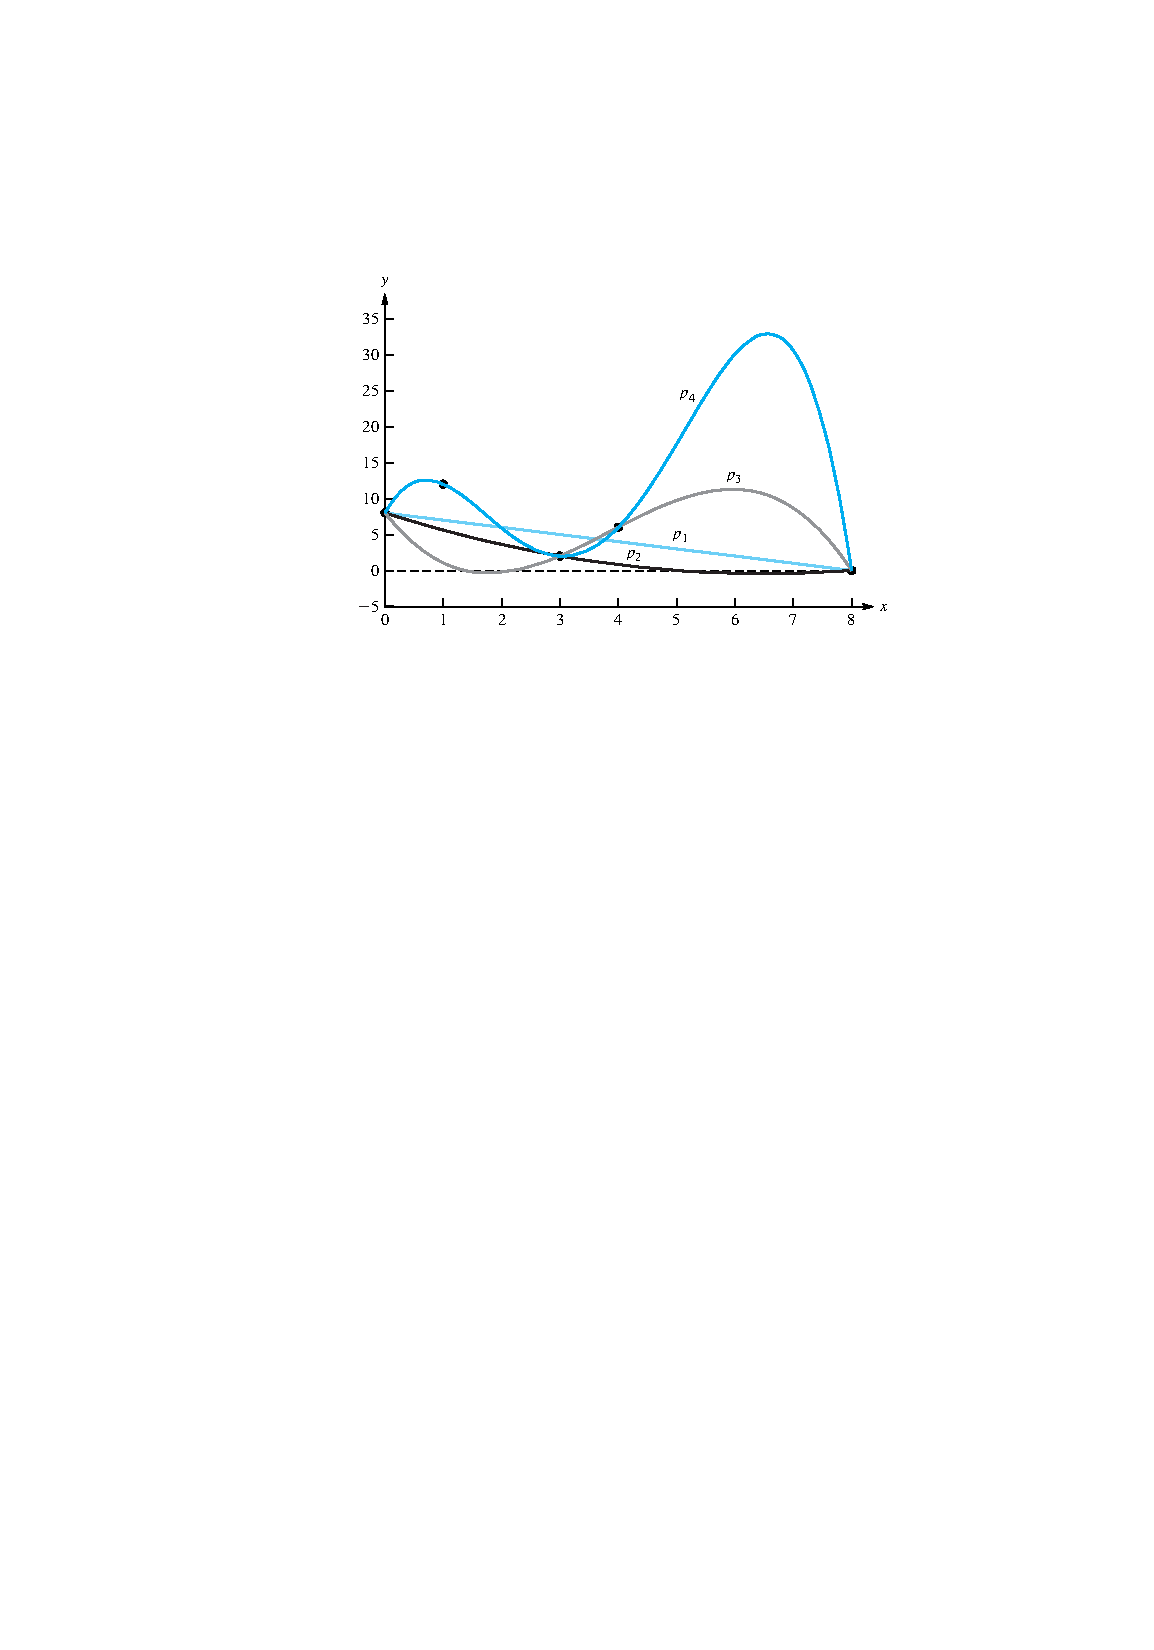
\includegraphics[width=0.5\textwidth]{Lec9_Fig5}}
\begin{itemize}
\item With more points added, the situation became \alert{worse} instead of better!
\item The reason is that  a polynomial of degree $n$ has $n$ zeros. 
If all of these zero points are real, then the curve crosses the $x$-axis $n$ times, resulting in \alert{wild oscillations}. 
\end{itemize}
\end{frame}
\begin{frame}{Errors in Polynomial Interpolation}
\begin{itemize}
\item  It can be shown that the error in polynomial interpolation is 
\[
f(x)-P_n(x)=\frac{(x-x_0)(x-x_1)\cdots(x-x_n)}{(n+1)!} f^{(n+1)}(\xi),
\]
where $\xi$ lies in the interval $(x_0, x_n)$.
\end{itemize}
\end{frame}

\begin{frame}{Warning}
\begin{itemize}
\item An interpolating polynomial intersecting more than \alert{six points} must be viewed with suspicion. 
\item The data points that are far from the point of interest do not contribute to the accuracy of the interpolating polynomial. 
\item  If \alert{extrapolation} using the interpolating polynomial is necessary, one should be careful.
\item \alert{Plot the data} and visually verify that the extrapolated value makes sense. 
\item	Use a \alert{low-order polynomial} based on nearest-neighbor data points. 
\item Work with a plot of $\log x$ vs. $\log y$, which is usually much smoother than the $x-y$
curve, and thus safer to extrapolate.
\end{itemize}
\end{frame}
%\begin{frame}{Cubic Spline}
%\begin{itemize}
%\item A \alert{spline function} is a function that consists of polynomial pieces joined together with certain smoothness conditions.
%\end{itemize}
%
%\begin{block}{Spline of degree $k$}
%A function $S$ is called a spline of degree $k$ if:
%\begin{itemize}
%\item The domain of $S$ is an interval$[a,b]$.
%\item  $S, S', S'', . . . , S^{(k-1)}$ are all continuous functions on $[a, b]$.
%\item There are points $t_i$ (the knots of $S$) such that $a=t_0 <t_1 < \cdots < t_n =b$ and such that $S$ is a polynomial of degree at most $k$ on each subinterval $[t_i , t_{i +1} ]$.
%\end{itemize}
%\end{block}
%
%\end{frame}
\subsection[Rational Function Interpolation]{Rational Function Interpolation}
\begin{frame}
\begin{itemize}
  \item   Some data are better interpolated by rational functions rather than polynomials.
  \item  A rational function $R(x)$ is a ratio of two polynomials:
  \[
    R(x) = \frac{P_m(x)}{Q_n(x)}=\frac{a_1 x^m+a_2 x^{m-1}+
    \cdots+a_m x+a_{m+1}}{b_1 x^n+b_2 x^{n-1}+\cdots+b_n x+b_{n+1}}
  \]
  \item We can rescale the coeffecients by setting  $b_{n+1}=1$ and this leaves $m+n+1$ undetermined 
  coefficients that must be computed by forcing $R(x)$ through $m+n+1$ data points.
  \item A popular version of $R(x)$ is the so-called diagonal rational function, where the degree of 
  the numerator is equal to that of the denominator $(m=n)$ if $m+n$ is even, or less by one ( $m=n-1$ ) if $m+n$ is odd. 
\end{itemize}
\end{frame}
\subsection[Cubic Spline Interpolation]{Cubic Spline Interpolation}
\begin{frame}
  \frametitle{Spline Interpolation}
  \begin{block}{Spline of degree $k$}
    A function $f$ is called a spline of degree $k$ if:
    \begin{enumerate}
    \item The domain of $f$ is an interval $[a, b]$.
    \item $f, f^{\prime}, f^{\prime \prime}, \ldots, f^{(k-1)}$ are all continuous functions on $[a, b]$.
    \item There are points $x_i$ (the knots of $f$ ) such that $a=x_0<x_1<\cdots<x_n=b$ and such that $f$ is a polynomial of degree at most $k$ on each subinterval $\left[x_i, x_{i+1}\right]$.
  \end{enumerate}
  \end{block}
  The most common spline is the \alert{cubic spline}, which is a piecewise cubic polynomial that is continuous in the first and second derivatives.
\end{frame}

\begin{frame}{Cubic Spline Interpolation}
  \centerline{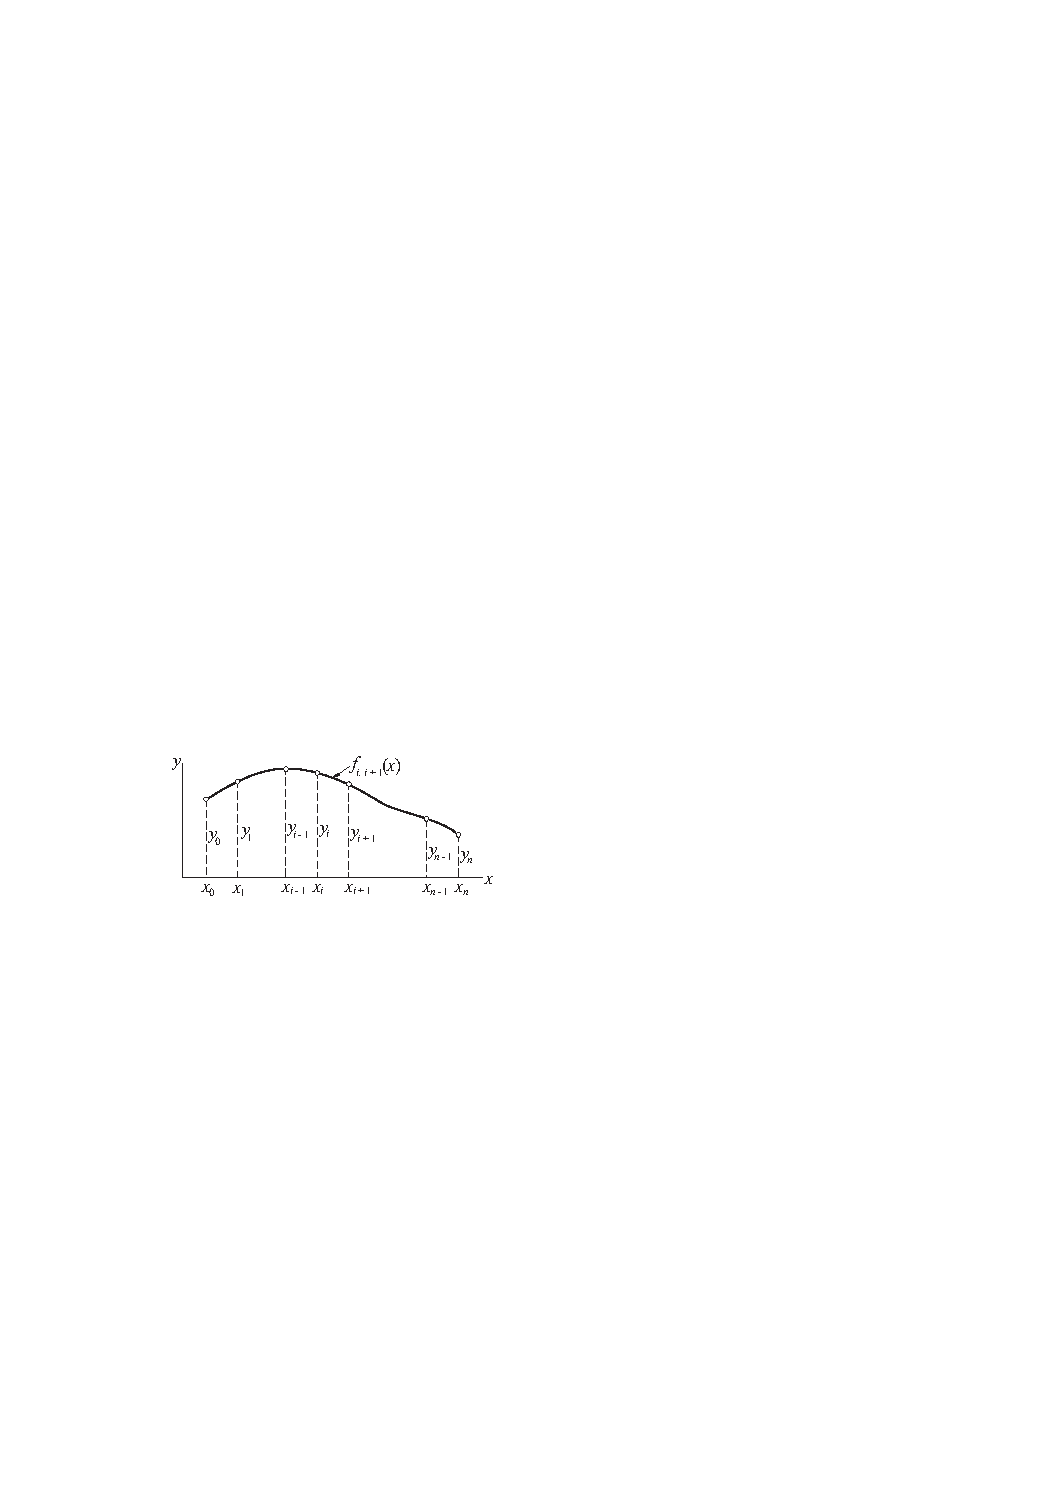
\includegraphics[width=0.5\textheight]{Lec9_Fig6.pdf}
   }
  
      \begin{itemize}
        \item A cubic spline is a piecewise cubic polynomial that is continuous in the first and second derivatives.
        \item   Denoting the second derivative of the spline at knot $i$ by $k_i$ , continuity of second derivatives requires that 
        \[
        f_{i-1, i}^{\prime \prime}\left(x_i\right)=f_{i, i+1}^{\prime \prime}\left(x_i\right)=k_i
        \]
        \item At the end points, we have the natural boundary conditions $k_0=k_n=0$.
      \end{itemize}
\end{frame}

\begin{frame}{Cubic Spline Algorithm}
  \begin{itemize}
    \item The starting point for computing the coefficients of $f_{i, i+1}(x)$ is the expression for $f_{i, i+1}^{\prime \prime}(x)$, which we know to be linear. 
    \item Using Lagrange's two-point interpolation, we can write  
    \[ 
    f_{i, i+1}^{\prime \prime}(x)=k_i \ell_i(x)+k_{i+1} \ell_{i+1}(x)
    \]
    where 
    \[
      \ell_i(x)=\frac{x-x_{i+1}}{x_i-x_{i+1}} \quad \ell_{1+1}(x)=\frac{x-x_i}{x_{i+1}-x_i}
    \]
    \item We have 
    \[ 
    f_{i, i+1}^{\prime \prime}(x)=\frac{k_i\left(x-x_{i+1}\right)-k_{i+1}\left(x-x_i\right)}{x_i-x_{i+1}}
    \]
  \end{itemize}
\end{frame}  
\begin{frame}{Cubic Spline Algorithm}
  \begin{itemize}
    \item Integration and use $f_{i, i+1}(x_i)=y_i$ to obtain
    \[ 
    \begin{aligned}
      f_{i, i+1}(x)= & \frac{k_i}{6}\left[\frac{\left(x-x_{i+1}\right)^3}{x_i-x_{i+1}}-\left(x-x_{i+1}\right)\left(x_i-x_{i+1}\right)\right] \\
      & -\frac{k_{i+1}}{6}\left[\frac{\left(x-x_i\right)^3}{x_i-x_{i+1}}-\left(x-x_i\right)\left(x_i-x_{i+1}\right)\right] \\
      & +\frac{y_i\left(x-x_{i+1}\right)-y_{i+1}\left(x-x_i\right)}{x_i-x_{i+1}}
      \end{aligned}
      \]
      
  \end{itemize}
\end{frame}  


\begin{frame}{Cubic Spline Algorithm}
  \begin{itemize}
  

  \item $k_i$ are determined by the condition that the slope   $f_{i-1, i}^{\prime}\left(x_i\right)=f_{i, i+1}^{\prime}\left(x_i\right)$  is continuous at $x_i$ for $i=1,2, \ldots, n-1$.
  \[
    \begin{aligned} 
      & k_{i-1}\left(x_{i-1}-x_i\right)+2 k_i\left(x_{i-1}-x_{i+1}\right)+k_{i+1}\left(x_i-x_{i+1}\right) \\ 
      = & 6\left(\frac{y_{i-1}-y_i}{x_{i-1}-x_i}-\frac{y_i-y_{i+1}}{x_i-x_{i+1}}\right), \quad i=1,2, \cdots, n-1
    \end{aligned}
  \]
   $k_i$ can be determined by solving a tridiagonal system of equations.
\end{itemize}
\end{frame}

\section[Numerical Differentiation]{Numerical Differentiation}
\subsection[Finite Difference Approximations]{Finite Difference Approximations}
\begin{frame}[fragile]
\frametitle{Numerical Differentiation: Introduction}
\begin{itemize}
\item Numerical differentiation deals with the following problem: given the function $y= f(x)$, obtain its derivatives at the point $x=x_k$.
\item The function is  usually given as a set of discrete data points $(x_i, y_i), i = 0,1,\ldots, n$, which can be the output of some computation or measurement.
\item One method to obtain numerical differentiation is through \alert{interpolation}. Approximate the function locally by a \alert{polynomial} and then differentiate it.
\item Another method is using \alert{finite difference} method based on  the Taylor series. 
\end{itemize}



\end{frame}

\begin{frame}[fragile]
\frametitle{Warning}
\begin{itemize}

\item Numerical differentiation is \alert{not} a particularly accurate process.
\item It suffers from  a conflict between \alert{ roundoff errors} (due to limited machine precision) and \alert{errors inherent in interpolation}. 
\item A derivative of a function can \alert{never} be computed with the same precision as the function itself.
\end{itemize}
\end{frame}

\begin{frame}[fragile]
\frametitle{Finite Difference Approximation}
\begin{itemize}
\item  Finite difference approximation is based on Taylor series expansion. It has the advantage of providing us with information about the \alert{error} involved in the approximation.

\item The derivation of the finite difference approximations for the derivatives of $f(x)$ is based on \alert{forward} and \alert{backward} Taylor series expansions of $f(x)$ about $x$.
\end{itemize}
\centerline{\includegraphics[width=0.8\textwidth]{Lec9_fig1}}
\end{frame}
\begin{frame}[fragile]
\frametitle{Taylor Series}
\begin{itemize}
\item The sums and differences of the series are given by 
\end{itemize}
\centerline{\includegraphics[width=0.6\textwidth]{Lec9_fig2}}
\begin{itemize}
\item The sums contain only \alert{even} derivatives, whereas the differences retain just the \alert{odd} derivatives.
\item These can be viewed as  simultaneous equations that can be solved for various derivatives of $f(x)$.
\end{itemize}
\end{frame}
%\subsection[First-Derivative Formula]{First-Derivative Formula}
\begin{frame}[fragile]
\frametitle{First-Derivative Formulas}
\begin{itemize}
\item The derivative for the function $f$ at $x_0$ is 
\[
f'(x_0)=\lim_{h\rightarrow 0} \frac{f(x_0+h)-f(x_0)}{h}
\]
\item The obvious method to approximate $f'(x_0)$ is 
\[
f'(x_0)\approx \frac{f(x_0+h)-f(x_0)}{h}
\]
for small values of $h$.
\end{itemize}
\end{frame}
\begin{frame}[fragile]
\frametitle{Error}
\begin{itemize}
\item To estimate the error in the finite difference approximation, we keep the order $h^2$ term in the Taylor expansion, 
\[
f(x_0+h)=f(x_0)+h f'(x_0)+\frac{1}{2}\,f''(\xi)h^2, 
\]
where $\xi$ is in the interval between $x_0$ and $x_0+h$.  
\item Rearranging, we have 
\[
f'(x_0)= \frac{f(x_0+h)-f(x_0)}{h}-\frac{1}{2}\,f''(\xi)h
\]
\item The \alert{truncation error} of our approximation is  $-\frac{1}{2}\,f''(\xi)h\sim O(h)$. This error will be present even if the calculations are performed with infinite precision. 
\item Additional  \alert{round-off errors} will be present when performing the calculation on a finite-precision machine.  
\end{itemize}
\end{frame}
\begin{frame}[fragile]
\frametitle{First Non-Central Difference Formulas}
%
\begin{itemize}
\item For positive $h$, we have the \alert{forward-difference formula}
\[
f'(x)=\frac{f(x+h)-f(x)}{h}+O(h)
\] 
and the \alert{backward-difference formula}
\[
f'(x)=\frac{f(x)-f(x-h)}{h}+O(h)
\]
\item The truncation error is of order $O(h)$. 
\end{itemize}
\end{frame}
\begin{frame}[fragile]
\frametitle{Higher Derivatives }
\begin{itemize}
\item  Approximations for higher derivatives can be derived in the same manner. 
\item The second derivative of $f(x)$ in the forward difference approximation is 
\[
f''(x)=\frac{f(x+2h)-2f(x+h)+f(x)}{h^2}+O(h).
\]
\item The truncation error is  of order $O(h)$. 
\item Higher order derivatives can be obtained in the same way.
\end{itemize}
\end{frame}
\begin{frame}[fragile]
\frametitle{Higher Derivatives:$O(h)$}

\begin{itemize}
\item Forward finite difference approximations of $O(h)$
\end{itemize}
\[\begin{array}{|c||r|r|r|r|r|}
  \hline & f(x) & f(x+h) & f(x+2 h) & f(x+3 h) & f(x+4 h) \\
  \hline \hline h f^{\prime}(x) & -1 & 1 & & & \\
  \hline h^2 f^{\prime \prime}(x) & 1 & -2 & 1 & & \\
  \hline h^3 f^{\prime \prime \prime}(x) & -1 & 3 & -3 & 1 & \\
  \hline h^4 f^{(4)}(x) & 1 & -4 & 6 & -4 & 1 \\
  \hline
  \end{array}
\]
%\centerline{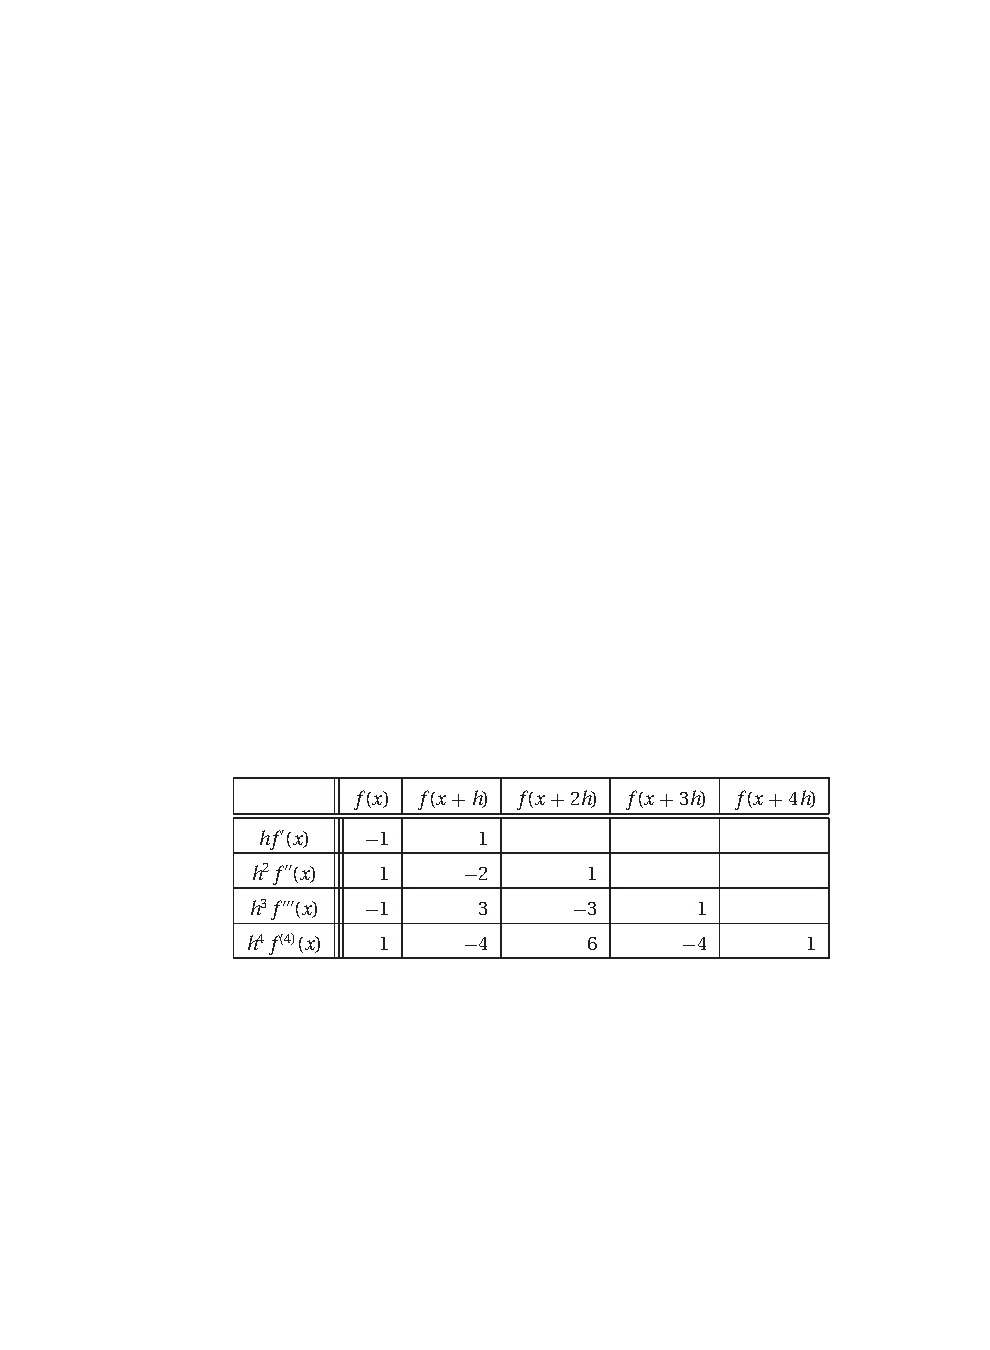
\includegraphics[width=0.8\textwidth]{Lec9_Tab1}}
\begin{itemize}
\item Backward finite difference approximations of $O(h)$
\end{itemize}
\[
\begin{array}{|c||r|r|r|r|r|}
  \hline & f(x-4 h) & f(x-3 h) & f(x-2 h) & f(x-h) & f(x) \\
  \hline \hline h f^{\prime}(x) & & & & -1 & 1 \\
  \hline h^2 f^{\prime \prime}(x) & & & 1 & -2 & 1 \\
  \hline h^3 f^{\prime \prime \prime}(x) & & -1 & 3 & -3 & 1 \\
  \hline h^4 f^{(4)}(x) & 1 & -4 & 6 & -4 & 1 \\
  \hline
\end{array}
\]
%\centerline{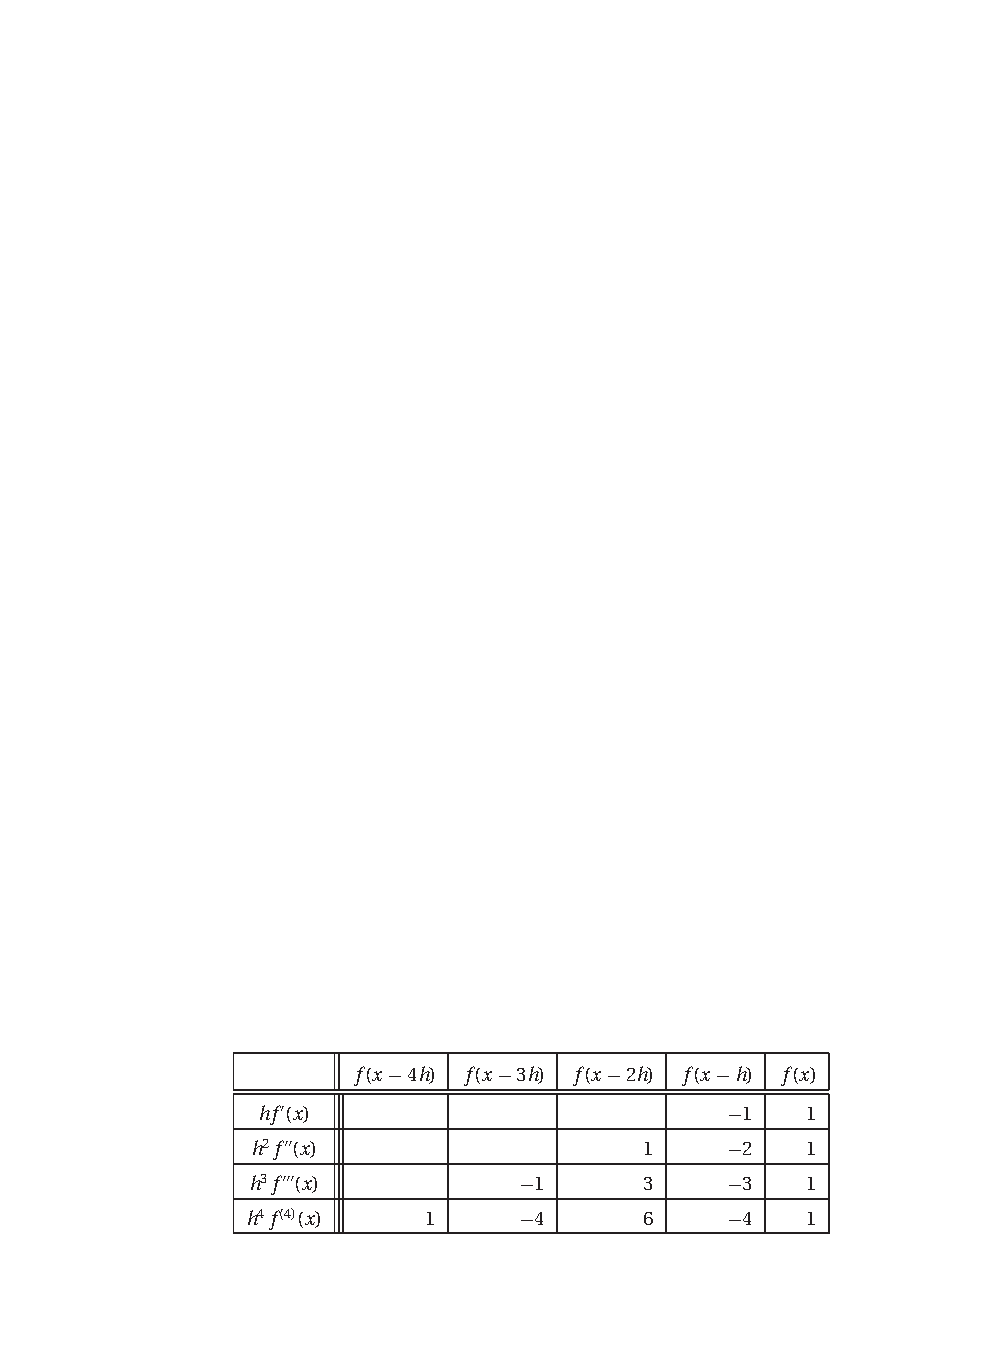
\includegraphics[width=0.8\textwidth]{Lec9_Tab2}}


\end{frame}

\begin{frame}[fragile]
\frametitle{First Central Difference Formulas}
\begin{itemize}
\item To improve the accuracy, one could combine the following two Taylor series
\begin{align}
f(x+h)&=f(x)+hf'(x)+\frac{h^2}{2!} f''(x)+ \frac{h^3}{3!} f'''(x)+\frac{h^4}{4!} f^{(4)}(x)+\cdots\nonumber\\
f(x-h)&=f(x)-hf'(x)+\frac{h^2}{2!} f''(x)- \frac{h^3}{3!} f'''(x)+\frac{h^4}{4!} f^{(4)}(x)+\cdots\nonumber
\end{align}
\item Subtracting them, we obtain the \alert{first central difference approximation} for $f'(x)$:
\[
f'(x)=\frac{f(x+h)-f(x-h)}{2h}+O(h^2)
\]
\item The truncation error is of order $O(h^2)$. 
\item This formula for numerical differentiation is very useful in the numerical solution of certain differential equations.
\end{itemize}
\end{frame}

\begin{frame}[fragile]
\frametitle{Higher Derivatives:$O(h^2)$}

\begin{itemize}
\item Second derivative is 
\[
f''(x)=\frac{f(x+h)-2f(x)+f(x-h)}{h^2}+O(h^2)
\]
\item The truncation error is of order $O(h^2)$.
\item Central finite difference approximations of $O(h^2)$:
\end{itemize}
%\centerline{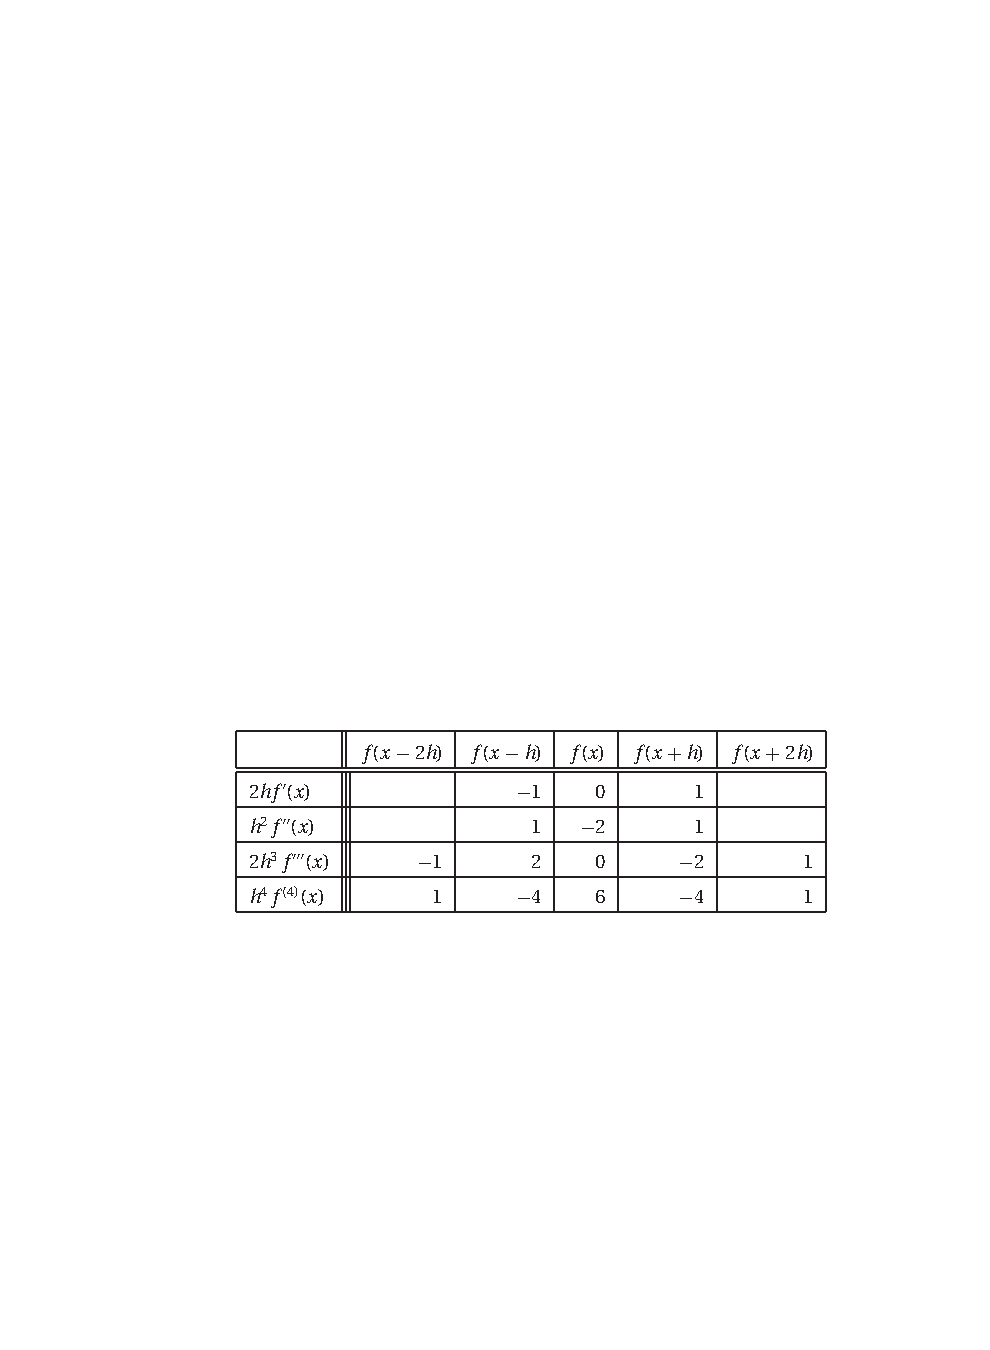
\includegraphics[width=0.8\textwidth]{Lec9_Tab3}}
\[
\begin{array}{|l|||r|r|r|r|r|}
  \hline & f(x-2 h) & f(x-h) & f(x) & f(x+h) & f(x+2 h) \\
  \hline \hline 2 h f^{\prime}(x) & & -1 & 0 & 1 & \\
  \hline h^2 f^{\prime \prime}(x) & & 1 & -2 & 1 & \\
  \hline 2 h^3 f^{\prime \prime \prime}(x) & -1 & 2 & 0 & -2 & 1 \\
  \hline h^4 f^{(4)}(x) & 1 & -4 & 6 & -4 & 1 \\
  \hline
\end{array}
\]
\end{frame}

\begin{frame}[fragile]
\frametitle{Second Non-Central Difference Formulas}
\begin{itemize}
\item For the forward or backward difference approximations, it is also preferable to use formulas with error of order $O(h^2)$.
\item For example, to obtain $f'(x)$, we use
\end{itemize}
\begin{align}
&f(x+h)=f(x)+hf'(x)+\frac{h^2}{2!} f''(x)+ \frac{h^3}{3!} f'''(x)+\frac{h^4}{4!} f^{(4)}(x)+\cdots\nonumber\\
&f(x+2h)=f(x)+2hf'(x)+2h^2 f''(x)+ \frac{4h^3}{3} f'''(x)+\frac{2h^4}{3} f^{(4)}(x)+\cdots\nonumber
\end{align}
\begin{itemize}
\item Eliminate $f''(x)$, we obtain the \alert{ second forward difference} formula,
\[
f'(x)=\frac{-f(x+2h)+4f(x+h)-3f(x)}{2h}+O(h^2)
\]
\item The truncation error is of order $O(h^2)$. 
\end{itemize}
\end{frame}
\begin{frame}[fragile]
\frametitle{Higher Derivatives: $O(h^2)$}

\begin{itemize}
\item Forward finite difference approximations of $O(h^2)$
\end{itemize}
\[
\begin{array}{|c||r|r|r|r|r|r|}
  \hline & f(x) & f(x+h) & f(x+2 h) & f(x+3 h) & f(x+4 h) & f(x+5 h) \\
  \hline \hline 2 h f^{\prime}(x) & -3 & 4 & -1 & & & \\
  \hline h^2 f^{\prime \prime}(x) & 2 & -5 & 4 & -1 & & \\
  \hline 2 h^3 f^{\prime \prime \prime}(x) & -5 & 18 & -24 & 14 & -3 & \\
  \hline h^4 f^{(4)}(x) & 3 & -14 & 26 & -24 & 11 & -2 \\
  \hline
\end{array}
\]
%\centerline{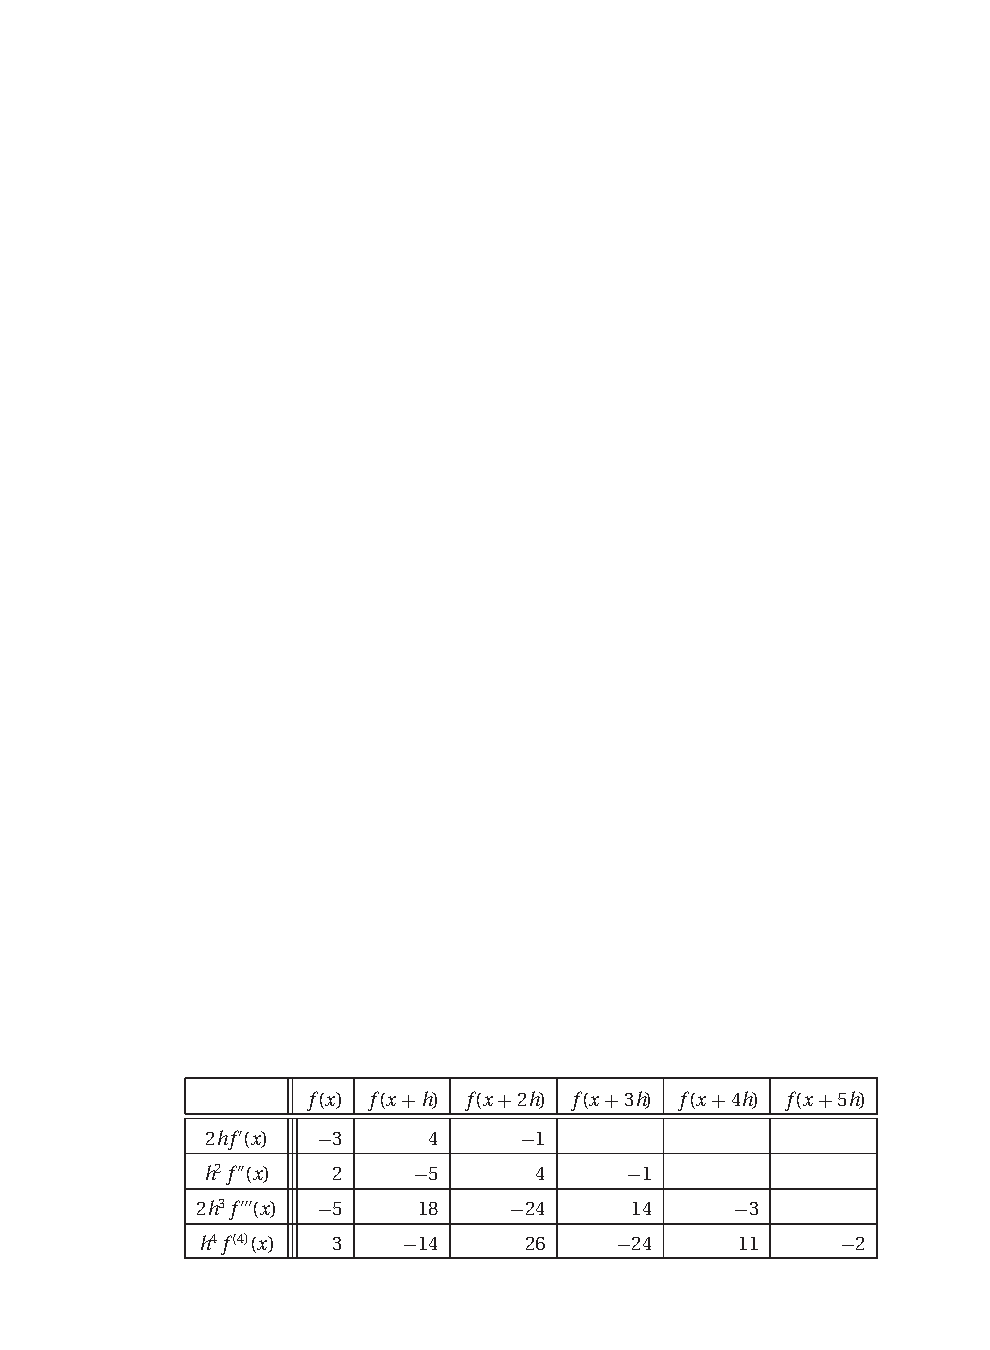
\includegraphics[width=0.8\textwidth]{Lec9_Tab4}}
\begin{itemize}
\item Backward finite difference approximations of $O(h^2)$
\end{itemize}
\[
\begin{array}{|c||r|r|r|r|r|r|}
  \hline & f(x-5 h) & f(x-4 h) & f(x-3 h) & f(x-2 h) & f(x-h) & f(x) \\
  \hline \hline 2 h f^{\prime}(x) & & & & 1 & -4 & 3 \\
  \hline h^2 f^{\prime \prime}(x) & & & -1 & 4 & -5 & 2 \\
  \hline 2 h^3 f^{\prime \prime \prime}(x) & & 3 & -14 & 24 & -18 & 5 \\
  \hline h^4 f^{(4)}(x) & -2 & 11 & -24 & 26 & -14 & 3 \\
  \hline
  \end{array}
\]
%\centerline{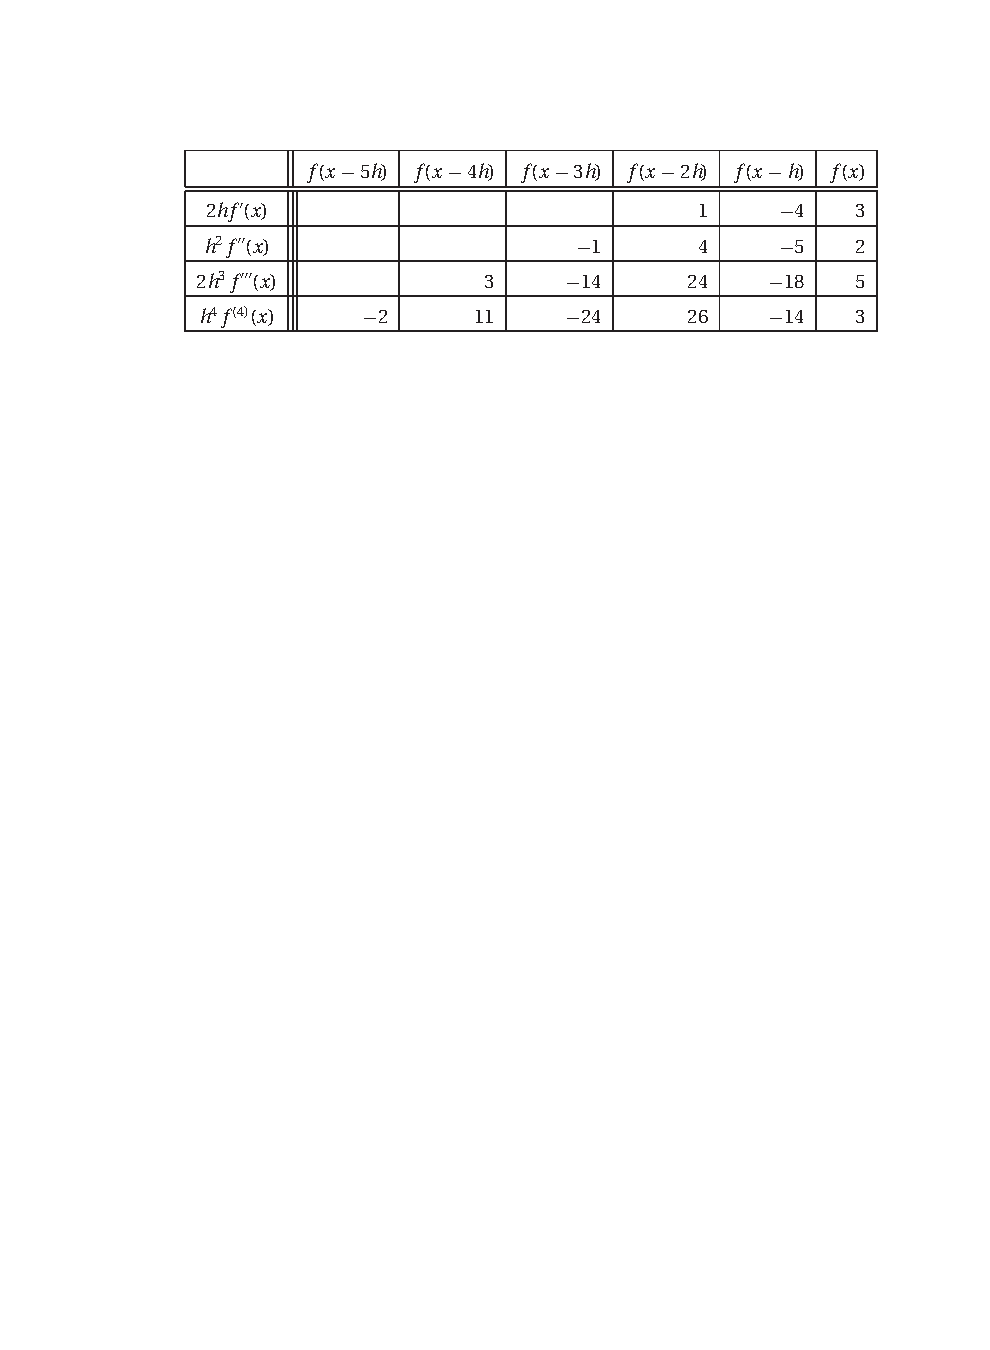
\includegraphics[width=0.8\textwidth]{Lec9_Tab5}}
\end{frame}
\begin{frame}{Errors in Finite Difference Approximations}
\begin{itemize}
\item The effect on since  in all finite difference expressions the sum of the coefficients is zero.
\item If $h$ is very small,  the values of $f(x), f(x\pm h), f(x\pm 2h)$, etc. will be approximately equal. The \alert{roundoff error} can be dominant and significant figures will be lost.
\item If $h$ is too big, the \alert{truncation errors} can dominate.
\item To minimize this problem, use double- or higher-precision arithmetics, and  employ finite difference formulas of $O(h^2)$.
 \end{itemize}
\end{frame}
\begin{frame}{Derivatives by Interpolation}
\begin{itemize}
\item If $f(x)$ is given as a set of discrete data points, interpolation can be a very effective means of computing its derivatives. 
\item The derivative of $f(x)$ is approximated by the derivative of the interpolant. 
\item This method is particularly useful if the data points are located at \alert{uneven intervals} of $x$, when the finite difference approximations discussed previously  are not applicable.
\end{itemize}
\end{frame}
\begin{frame}{Polynomial Interpolant}
\begin{itemize}
\item We want to fit the data to the polynomial of degree $n$
\[
P_{n-1}(x)=a_0+a_1 x+ a_2 x^2+a_3 x^3+\cdots +a_nx^n
\]
through $n+1$ data points and evaluate its derivative.
\item The degree of the polynomial is limited to less than 6 in order to avoid spurious \alert{oscillations} of the interpolant. 
\item These oscillations are \alert{magnified} with each differentiation.
\item The interpolation should be a local one, involving no more than a few nearest-neighbor data points.
\item When the data is noisy, it is advisable to use the \alert{least-squares fit} to find the best fitting polynomial.  
\end{itemize}
\end{frame}
\begin{frame}{First-Derivative Formulas via Interpolation Polynomial}
\begin{itemize}
%\item If the function $f$ is approximated by $p$ so that $f \approx p$. We can obtain the derivative of $f'(x)\approx p'(x)$.
%\item In practice, we want to determine $p$ by interpolation of a few points. 
\item If $p$ is the polynomial of degree $\le 1$ that interpolate $f$ at two nodes $x_1$, $x_2$, 
\[ 
p_1(x)=f(x_1)+\frac{f(x_2)-f(x_1)}{x_2-x_1}(x-x_1)=f(x_1)+f[x_1,x_2](x-x_1)
\]
\item The first derivative 
\[
f'(x)\approx p_1'(x)=f[x_1,x_2]=\frac{f(x_2)-f(x_1)}{x_2-x_1}.
\]
\item Interpolation through 3 nodes $x_1,x_2, x_3$,
\[
p_2(x)=f(x_1)+f[x_1,x_2] (x-x_1)+f[x_1,x_2,x_3](x-x_1)(x-x_2)
\]
where $f[x_1,x_2,x_3]=(f[x_2,x_3]-f[x_1,x_2])/(x_3-x_1)$. 
\item The first derivative
\[
f'(x)\approx p_2'(x)=f[x_1,x_2]+f[x_1,x_2,x_3](2x-x_1-x_2).
\]
\end{itemize}
\end{frame}
\subsection[Richardson's Extrapolation]{Richardson's Extrapolation}
\begin{frame}{Richardson's Extrapolation}
\begin{itemize}
\item Richardson's extrapolation is a method to generate \alert{high-accuracy results} using \alert{low-order formulas}. 
\item For a given quantity $G$, if we can approximate it by $g(h)$, which depends on $h$, with an error $E(h)=ch^p$, where $c$ and $p$ are constants, such that, 
\[
G=g(h)+E(h).
\]
\item For a given  $h=h_1$,  
$G=g(h_1)+ch_1^p$, and for $h=h_2$, $G=g(h_2)+ch_2^p$.
\item Eliminating $c$ and solving for $G$, we obtain the \alert{Richardson extrapolation formula},
\[
G=\frac{\left(\frac{h_1}{h_2}\right)^p g(h_2)-g(h_1)}{\left(\frac{h_1}{h_2}\right)^p-1}.
\]

 
\end{itemize}
\end{frame}
\begin{frame}{Application to Differentiation}
\begin{itemize}
\item It is common practice to choose $h_2=h_1/2$, and
\[
G=\frac{2^p g(h_1/2)-g(h_1)}{2^p-1}.
\]
\item Consider the central difference formula
\begin{align*}
f'(x)&=\frac{f(x+h)-f(x-h)}{2h}+a_2h^2+a_4h^4+a_6h^6+\ldots\\
&=\phi(h)+a_2h^2+a_4h^4+a_6h^6+\ldots
\end{align*}
\item $\phi(h)=\frac{f(x+h)-f(x-h)}{2h}$ is an approximation to $f'(x)$ with an error of order $O(h^2)$.
\end{itemize}
\end{frame}
\begin{frame}{Central Difference Approximation}
\begin{itemize}
\item Evaluate $\phi$ at $h$ and $h/2$,
\begin{align*}
\phi(h)&=f'(x)-a_2h^2-a_4h^4-a_6h^6-\ldots\\
\phi\left(\frac{h}{2}\right)&=f'(x)-a_2\left(\frac{h}{2}\right)^2-a_4\left(\frac{h}{2}\right)^4-a_6\left(\frac{h}{2}\right)^6-\ldots
\end{align*}
\item Eliminate the dominant error term $O(h^2)$, 
\[
\phi\left(\frac{h}{2}\right)+\frac{1}{3}\left[\phi\left(\frac{h}{2}\right)-\phi(h)\right]=f'(x)+\frac{1}{4}a_4h^4+\frac{5}{16}a_6h^6+\cdots
\]
\item The precision is improved to $O(h^4)$ because the error series of the new combination begins with $\frac{1}{4} a_4h^4$.

 \end{itemize}
\end{frame}
\begin{frame}{Improved Precision}
\begin{itemize}
\item Define 
\[
\Phi(h)=\phi\left(\frac{h}{2}\right)+\frac{1}{3}\left[\phi\left(\frac{h}{2}\right)-\phi(h)\right]
\]
\item Repeat the process, we obtain
\[
\Phi\left(\frac{h}{2}\right)+\frac{1}{15}\left[\Phi\left(\frac{h}{2}\right)-\Phi(h)\right]=f'(x)-\frac{1}{20}b_6h^6+\cdots
\]
\item The precision is improved to $O(h^6)$.
\item The same procedure can be \alert{repeated over and over again} to kill higher and higher terms in the error. 
 \end{itemize}
\end{frame}
\begin{frame}{General Form}
\begin{itemize}
\item Let $N(h)$ be a function which approximates an unknown $M$, such that
\[
M=N(h)+\sum_{k=1}^{\infty} a_{k} h^{k}.
\]
\item Assumed that $N(h)$ can be computed for any $h>0$, so 
\[
M=N\left(\frac{h}{2}\right)+\sum_{k=1}^{\infty} a_{k} \left(\frac{h}{2}\right)^{k}.
\]
\item Eliminate the term involving $a_1$, 
\[
M=\left[2N_1\left(\frac{h}{2}\right)-N_1(h)\right]+a_2 \left(\frac{h^2}{2}-h^2\right)+a_3 \left(\frac{h^3}{4}-h^3\right)+\cdots,
\]
where $N_1(h)\equiv N(h)$.
\end{itemize}
\end{frame}
\begin{frame}{General Form }
\begin{itemize}
\item Define 
\[
N_2(h)=\left[2N_1\left(\frac{h}{2}\right)-N_1(h)\right]=N_1\left(\frac{h}{2}\right)+\left[N_1\left(\frac{h}{2}\right)-N_1(h)\right]
\]
and we obtain the $O(h^2)$ approximation formula ,
\[
M=N_2(h)-\frac{a_2}{2}h^2-\frac{3a_3}{4}h^3-\cdots.
\]
\item Repeat the process again, we obtain the $O(h^3)$ formula,
\begin{align*}
M &=\left[N_2\left(\frac{h}{2}\right)-\frac{N_2\left(\frac{h}{2}\right)-N_2(h)}{3}\right]+\frac{a_3}{8}h^3+\cdots\\
 &= N_3(h)+\frac{a_3}{8}h^3+\cdots.
\end{align*}
\end{itemize}
\end{frame}
\begin{frame}{General Form }
\begin{itemize}
\item The process can be repeated to construct an $O(h^4)$ approximation, 
\[
N_4(h)=N_3\left(\frac{h}{2}\right)+\frac{N_3\left(\frac{h}{2}\right)-N_3(h)}{7},
\]
and  $O(h^5)$ approximation ,
\[
N_5(h)=N_4\left(\frac{h}{2}\right)+\frac{N_4\left(\frac{h}{2}\right)-N_4(h)}{15}.
\]
\end{itemize}
\end{frame}
\begin{frame}{General Form }
\begin{itemize}
\item In general, if $M$ can be written as
\[
M=N(h)+\sum_{j=1}^{m-1} a_j h^j +O(h^m)
\]
then for each $j=2,3,\cdots m$, we have an $O(h^j)$ approximation of the form
\[
N_j(h)=N_{j-1}\left(\frac{h}{2}\right)+\frac{N_{j-1}\left(\frac{h}{2}\right)-N_{j-1}(h)}{2^{j-1}-1}.
\]
\end{itemize}
\end{frame}
\begin{frame}{General Form}
\begin{itemize}
\item The approximations are generated by rows in the order indicated in the following table ($N_1(h)\equiv N(h)$):
\end{itemize}
\begin{center}
\begin{tabular}{llll}
\hline
$O(h)$ & $O(h^2)$ & $O(h^3)$ & $O(h^4)$\\
\hline
1: $N_1(h) $ & & & \\
2: $N_1\left(\frac{h}{2}\right) $ & 3: $N_2(h)$ & & \\
4: $N_1\left(\frac{h}{4}\right) $ & 5: $N_2\left(\frac{h}{2}\right)$ & 6: $N_3(h)$& \\
7: $N_1\left(\frac{h}{8}\right) $ & 8: $N_2\left(\frac{h}{4}\right)$ & 9: $N_3\left(\frac{h}{2}\right)$& 10:$N_4(h)$\\
\hline

\end{tabular}
\end{center}
\end{frame}
\end{document}


